\documentclass[tikz,border=10pt]{standalone}
\usepackage{circuitikz}
\usepackage{xcolor}
\usepackage{amsmath}
\usetikzlibrary{arrows, decorations.pathmorphing, shapes.symbols}

\begin{document}
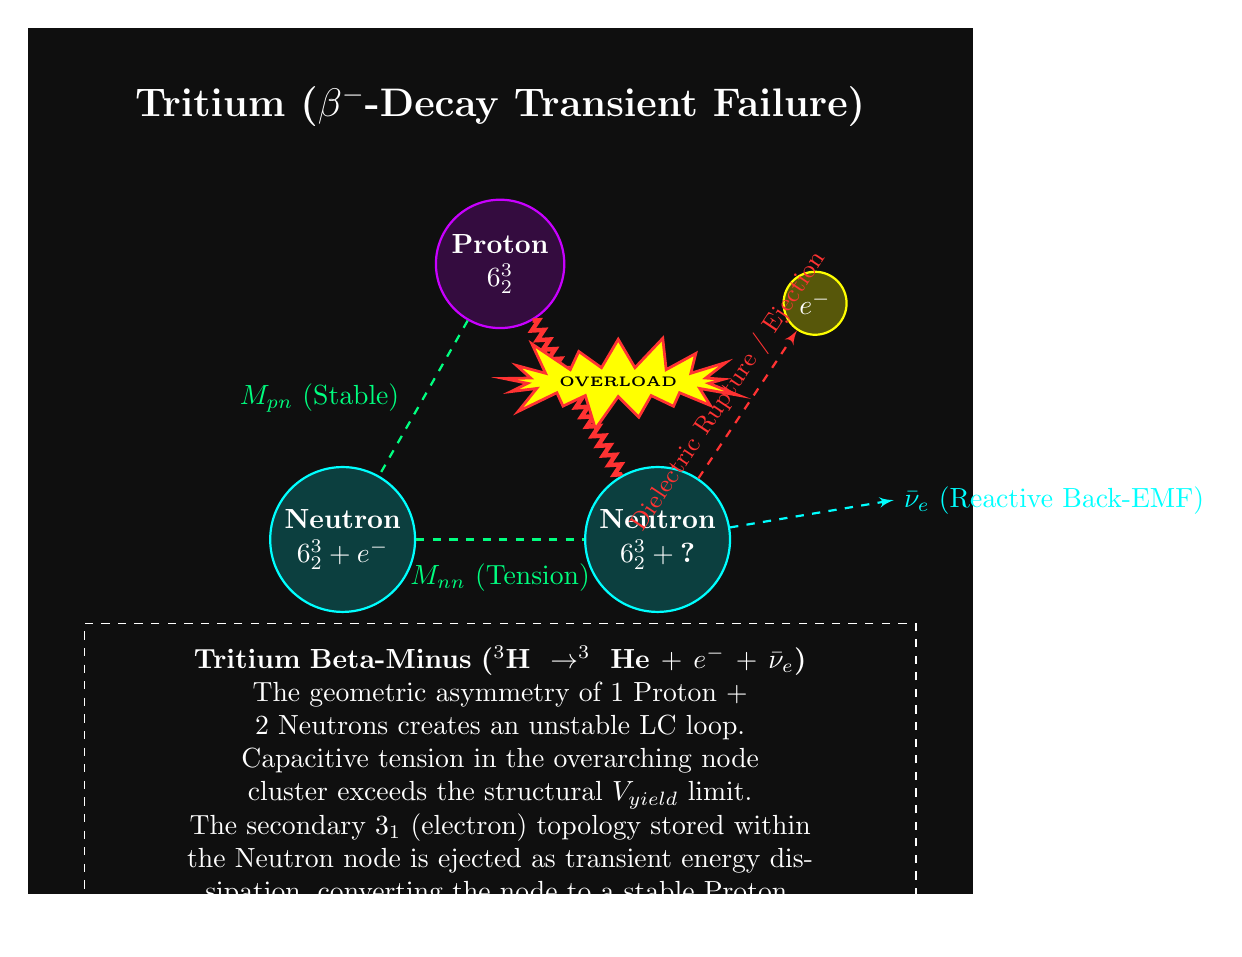
\begin{tikzpicture}[>=latex']

\definecolor{neonblue}{RGB}{0, 255, 255}
\definecolor{neongreen}{RGB}{0, 255, 128}
\definecolor{neonred}{RGB}{255, 50, 50}
\definecolor{neonpurple}{RGB}{200, 0, 255}
\definecolor{darkbg}{RGB}{15, 15, 15}
\definecolor{neonyellow}{RGB}{255, 255, 0}

% Fill background
\fill[darkbg] (-6,-6) rectangle (6,5);

% Title
\node[text=white, font=\bfseries\Large] at (0, 4) {Tritium ($\beta^-$-Decay Transient Failure)};

\tikzset{
    proton block/.style={
        draw=neonpurple, thick, fill=darkbg!80!neonpurple,
        circle, inner sep=2pt,
        minimum size=1.5cm,
        text=white, font=\bfseries, align=center
    },
    neutron block/.style={
        draw=neonblue, thick, fill=darkbg!80!neonblue,
        circle, inner sep=2pt,
        minimum size=1.5cm,
        text=white, font=\bfseries, align=center
    },
    electron/.style={
        draw=neonyellow, thick, fill=neonyellow!30!darkbg,
        circle, inner sep=1pt,
        minimum size=0.8cm,
        text=white, font=\bfseries, align=center
    },
    bus/.style={
        draw=neongreen, thick, dashed
    },
    rupture/.style={
        draw=neonred, ultra thick, decoration={zigzag, segment length=4pt, amplitude=2pt}, decorate
    }
}

% Tritium Nucleons (1 Proton, 2 Neutrons in an unstable triad)
\node[proton block] (P1) at (0, 2) {Proton\\$6^3_2$};
\node[neutron block] (N1) at (-2, -1.5) {Neutron\\$6^3_2 + e^-$};
\node[neutron block] (N2) at (2, -1.5) {Neutron\\$6^3_2 + \text{?}$};

% Intact Couplings
\draw[bus] (P1) -- (N1) node[midway, left=5pt, text=neongreen] {$M_{pn}$ (Stable)};
\draw[bus] (N1) -- (N2) node[midway, below=5pt, text=neongreen] {$M_{nn}$ (Tension)};

% Rupturing Coupling (Beta Decay specific)
\draw[rupture] (P1) -- (N2);

% Rupture Explosion Star on N2
\node[starburst, fill=neonyellow, draw=neonred, line width=1pt, inner sep=2pt, font=\bfseries\tiny, text=black] at (1.5, 0.5) {OVERLOAD};

% Ejection Path
\node[electron] (E) at (4, 1.5) {$e^-$};
\draw[->, neonred, thick, dashed] (N2) -- (E) node[midway, sloped, above, text=neonred, font=\small] {Dielectric Rupture / Ejection};

% Beta Decay Anti-neutrino representation
\coordinate (Nu) at (5, -1);
\draw[->, neonblue, thick, dashed] (N2) -- (Nu) node[right, text=neonblue] {$\bar{\nu}_e$ (Reactive Back-EMF)};

% Annotations
\node[text=white, text width=10cm, align=center, draw=white, dashed, inner sep=8pt] at (0, -4.5) {
    \textbf{Tritium Beta-Minus ($^3\text{H} \rightarrow ^3\text{He} + e^- + \bar{\nu}_e$)}\\
    The geometric asymmetry of 1 Proton + 2 Neutrons creates an unstable LC loop.\\
    Capacitive tension in the overarching node cluster exceeds the structural $V_{yield}$ limit.\\
    The secondary $3_1$ (electron) topology stored within the Neutron node is ejected as transient energy dissipation, converting the node to a stable Proton.
};

\end{tikzpicture}
\end{document}
